\chapter{Iteración 7}

\begin{quotation}[Aerospace Engineer]{Burt Rutan (1943--)}
Testing leads to failure, and failure leads to understanding.
\end{quotation}

\begin{abstract}
Esta iteración se orienta a consolidar sistemas ya introducidos y a extender la estructura
del recorrido con salas especiales. El trabajo integra la sala de tienda y la lógica base
de las salas secreta y de tesoro dentro de la generación procedural del mapa, además de
refinar el sistema de combate y el sistema de enemigos.
\end{abstract}

\section{Análisis de características}
La séptima iteración se plantea como una fase de consolidación sobre sistemas que en la
entrega anterior ya eran funcionales, pero todavía admitían una mejora clara en profundidad
jugable y en variedad de recorrido. La incorporación de salas especiales amplía la
estructura del mapa con espacios de función diferenciada, mientras que el refinamiento de
combate y enemigos mejora la respuesta táctica de los encuentros. En el estado actual del
proyecto, la parte más cerrada de la iteración corresponde al refinamiento de combate y
enemigos, mientras que las salas especiales quedan ya encajadas a nivel estructural y
visual, aunque todavía requieren cierre funcional para darse por terminadas del todo.

\begin{enumerate}
\item \textbf{Sala Tienda.} Esta funcionalidad introduce una habitación especial dentro
de la generación del mapa con identidad propia y con señalización específica en el minimapa.
En el estado actual de la iteración, su aporte principal consiste en quedar integrada dentro
del reparto de salas terminales, contar con tipo de sala diferenciado y poder representarse
de forma explícita tanto en la celda del mapa como en la configuración de puertas y muros.
Aunque su comportamiento jugable todavía necesita cerrarse, esta base ya permite tratar la
tienda como una categoría espacial propia dentro de la estructura procedural del nivel.

\item \textbf{Sala Secreta y Tesoro.} Esta funcionalidad amplía la distribución de salas
especiales con espacios que no siguen exactamente las mismas reglas de acceso que las salas
regulares. La implementación actual ya distingue estos nodos dentro del mapa, les asigna
iconografía propia y, en el caso de la sala secreta, evita su conexión directa mediante el
flujo habitual de puertas visibles. Esto refuerza la idea de exploración y de recompensa por
descubrimiento, aunque el cierre definitivo de su comportamiento y de su contenido todavía
queda pendiente dentro del desarrollo posterior de la iteración.

\item \textbf{Sistema de Combate II.} Esta funcionalidad refina el combate del jugador para
que cada arma no solo tenga parámetros distintos, sino también una lectura más clara en su
uso y una interacción más rica con el resto de sistemas. El trabajo realizado en esta
iteración introduce ataques cargados para armas que lo requieren, proyectiles con
comportamiento más sofisticado y apoyo visual específico tanto en ataques cuerpo a cuerpo
como en proyectiles. Además, el sistema mantiene el contexto del arma y de la forma activa
del jugador durante el ataque, lo que facilita que otros componentes interpreten el impacto
con mayor precisión. En la práctica, esta ampliación hace que el combate se perciba como un
sistema más expresivo, con mejor retroalimentación y con una conexión más sólida entre
entrada, ataque y efecto producido en pantalla.

\item \textbf{Sistema de Enemigos II.} Esta funcionalidad profundiza en el comportamiento
enemigo sobre la base ya creada anteriormente. Su alcance real consiste en diferenciar con
más claridad la respuesta táctica de cada arquetipo, introduciendo preparación visible del
ataque, desplazamientos de compromiso, recuperación tras empujes y una relación más fuerte
entre el contexto del arma del jugador y el daño final que recibe cada tipo de enemigo. A
esto se suma una mejor activación por sala y una integración más coherente con el sistema de
aparición ponderada por círculo y por tipo de habitación. En términos funcionales, la
feature hace que los enfrentamientos resulten más legibles y menos genéricos, ya que el
jugador puede anticipar mejor la intención del enemigo y adaptar su respuesta según el tipo
de amenaza al que se enfrenta.

La combinación de estas funcionalidades hace que la séptima iteración actúe como una capa de
consolidación y ampliación. Por un lado, refuerza la calidad táctica del combate y de los
enemigos; por otro, abre el mapa a recorridos más variados mediante salas especiales con un
papel diferenciado dentro de la partida.

\section{Diseño}
El diseño de esta iteración parte de una necesidad doble: enriquecer la calidad de los
enfrentamientos y dar más valor estructural a determinadas salas dentro del recorrido
procedural. En ambos casos, la idea dominante fue evitar soluciones aisladas y reutilizar la
arquitectura ya existente para hacerla más expresiva sin perder coherencia con lo anterior.

\subsection{Diseño de Sala Tienda}
La sala de tienda se diseñó como una categoría espacial propia dentro del conjunto de salas
terminales del mapa. La decisión importante aquí fue integrarla en la misma fase de
selección procedural que otras salas especiales, en lugar de tratarla como una excepción
colocada manualmente después.

Este enfoque hace que la tienda forme parte natural del reparto del recorrido y permite que
su identidad visual y estructural quede resuelta desde el propio generador de mapa, aunque
la lógica jugable específica que contendrá la sala todavía deba completarse.

\subsection{Diseño de Sala Secreta y Tesoro}
La lógica de estas salas se diseñó para reforzar la exploración y la recompensa. La sala de
tesoro se concibe como un nodo especial identificado dentro del mapa, mientras que la sala
secreta requiere además un tratamiento distinto en su accesibilidad para que su descubrimiento
no se perciba igual que el de una habitación regular.

Por ello, el diseño introduce tipos de sala específicos y reglas de conexión diferenciadas,
de forma que la presencia de estas habitaciones no solo cambie el icono mostrado en el mapa,
sino también la lectura espacial del recorrido.

\subsection{Diseño de Sistema de Combate II}
El refinamiento del combate se diseñó bajo el criterio de mantener una lógica unificada para
todas las armas, pero permitiendo comportamientos suficientemente distintos como para que la
elección de una u otra tenga consecuencias jugables reales. A partir de ahí, se incorporó la
idea de ataques cargados y de proyectiles con capacidades adicionales, sin romper el modelo
de arma configurable que ya existía.

También se dio importancia al \textit{feedback} visual del ataque. Si el sistema pretendía
ser más expresivo, la respuesta en pantalla debía acompañar ese aumento de complejidad. Por
eso, el diseño no se limita a parámetros de daño o alcance, sino que contempla también
trazos, partículas y apoyos visuales ligados a la ejecución del ataque \cite{gameendeavorCombatFun}.

\subsection{Diseño de Sistema de Enemigos II}
La decisión principal fue reforzar la identidad táctica de cada tipo de enemigo mediante
patrones de ataque y movimiento más distinguibles. No bastaba con que hubiera variantes con
distinto daño o velocidad; era necesario que el jugador percibiera de forma clara cuándo un
enemigo iba a cargar, disparar o comprometer una embestida.

Por ello, el diseño de esta ampliación se orientó a introducir fases de preparación visibles,
desplazamientos de ataque más marcados y una respuesta al daño más sensible al arma empleada.
Con ello, el enemigo deja de ser únicamente una fuente de daño y pasa a actuar como una
pieza táctica reconocible dentro del encuentro.

\section{Implementación}
La implementación de esta iteración se repartió entre el refinamiento de sistemas de acción
y la ampliación del generador procedural con nuevos tipos de sala. Aunque a nivel funcional
las features parecen distintas, todas comparten un mismo objetivo: hacer que el juego
responda con más riqueza al contexto en el que se produce cada evento.

\subsection{Implementación de Sala Tienda}
La base técnica de la sala de tienda se apoya en \texttt{MapGenerator}, \texttt{Cell} y en
la configuración de puertas y muros de \texttt{Room}. \texttt{MapGenerator} selecciona un
índice específico para esta sala dentro del conjunto de habitaciones terminales, le asigna
un tipo propio y actualiza su representación visual en el mapa mediante iconografía
dedicada.

Después, esa información se propaga al resto del sistema a través del tipo de sala
almacenado en la celda, lo que permite que puertas, muros y minimapa la interpreten como una
categoría distinta. Aunque el contenido interactivo definitivo de la tienda no está cerrado,
la integración estructural de la sala sí queda resuelta en esta fase.

La Figura~\ref{fig:iteracion7-feature-tienda} muestra el resultado visual de esta integración.


\subsection{Implementación de Sala Secreta y Tesoro}
La incorporación de salas especiales se apoya también en \texttt{MapGenerator}, que reserva
índices específicos para estas habitaciones y actualiza su \texttt{RoomType} dentro de cada
\texttt{Cell}. En el caso de la sala secreta, la selección se realiza con una lógica propia
que busca posiciones no ocupadas y con suficiente proximidad estructural al resto del mapa
para poder insertarla como espacio oculto.

Por otra parte, \texttt{Room} utiliza el tipo de sala para condicionar la colocación de
puertas. Esto permite que la sala secreta no siga exactamente el mismo patrón de acceso que
una sala regular, reforzando su papel como espacio de descubrimiento. La sala de tesoro
queda igualmente integrada en el sistema de identificación y representación, aunque su
acabado funcional completo todavía sigue abierto.

La Figura~\ref{fig:iteracion7-feature-salas-especiales} recoge el resultado obtenido para estas salas especiales.


\subsection{Implementación de Sistema de Combate II}
El refinamiento del combate se apoya en \texttt{PlayerCombatController},
\texttt{WeaponDefinition}, \texttt{Projectile}, \texttt{MeleeHitbox},
\texttt{PlayerChargeAttackVisual} y los componentes visuales asociados a proyectiles y
golpes de melé. \texttt{PlayerCombatController} mantiene la selección de arma según la forma
del jugador y amplía el flujo de ataque para soportar ataques cargados, donde el daño final
depende del tiempo de preparación acumulado.

En paralelo, la implementación añade apoyo visual para hacer más legible cada acción:
trazos de ataque en melé, indicadores de carga y estelas o partículas ligadas al
desplazamiento de proyectiles. El sistema conserva además el contexto completo del ataque
mediante \texttt{DamageSourceContext}, lo que permite conectar el golpe con otros sistemas
que interpretan el impacto más allá del valor numérico del daño.

La Figura~\ref{fig:iteracion7-feature-combate} muestra el resultado de este refinamiento del combate.


\subsection{Implementación de Sistema de Enemigos II}
La ampliación del comportamiento enemigo se apoyó sobre todo en \texttt{EnemyController},
\texttt{EnemyProjectile}, \texttt{EnemyHealth} y \texttt{CircleDefinition}. En
\texttt{EnemyController} se refuerzan los patrones diferenciados de enemigos normales,
voladores y tanque mediante tiempos de preparación, ataques con embestida, disparos a
distancia, recuperación de \textit{knockback} y señales visuales previas al ataque.

Además, el sistema se integra de forma más estrecha con el contexto del arma del jugador.
Para ello se consulta \texttt{DamageSourceContext}, lo que permite ajustar multiplicadores de
daño en función del arma concreta y de la forma activa. A esto se suma una mejor relación
con la activación por sala, el estado dormido inicial y la selección ponderada de enemigos
desde la definición del círculo y del tipo de habitación.

El resultado visual de esta ampliación del comportamiento enemigo puede verse en la Figura~\ref{fig:iteracion7-feature-enemigos}.

\end{enumerate}

\section{Pruebas}
Las pruebas realizadas en esta iteración se centraron en validar tanto la ampliación del
recorrido con salas especiales como el refinamiento táctico de combate y enemigos. La Tabla~\ref{tab:iteracion7-pruebas}
siguiente resume los playtests manuales que se ejecutaron para comprobar tienda, salas
secreta y de tesoro, ataques cargados y nuevos patrones enemigos.

Además, estas pruebas fueron útiles para encontrar errores concretos en la configuración de
las salas especiales, tanto en tienda como en tesoro y sala secreta. También permitieron
detectar ajustes necesarios en algunos elementos interactivos asociados a estas habitaciones,
mejorando su coherencia espacial y funcional dentro del recorrido.

\begin{table}[H]
    \centering
    \begin{coolTable}{p{.27\textwidth}p{.62\textwidth}}{2}
    {Pruebas de playtest realizadas en la iteración 7}
    \textbf{Feature bajo Test} & \textbf{Descripción de la prueba realizada} \\
    \midrule
    Sala Tienda & \begin{minipage}[t]{\linewidth}\begin{enumerate}\item Generar partidas hasta localizar la tienda. \item Entrar y observar su representación en el minimapa. \item Verificar que aparece como sala terminal diferenciada y que conserva puertas y muros coherentes.\end{enumerate}\end{minipage} \\
    \midrule
    Sala Secreta y Tesoro & \begin{minipage}[t]{\linewidth}\begin{enumerate}\item Generar partidas con salas especiales. \item Localizar tesoro y sala secreta. \item Verificar su iconografía propia, que la secreta no se muestre como una sala regular y que ambas no rompan la navegación.\end{enumerate}\end{minipage} \\
    \midrule
    Sistema de Combate II & \begin{minipage}[t]{\linewidth}\begin{enumerate}\item Probar armas normales y cargadas en combate. \item Observar trazos, indicadores y proyectiles. \item Confirmar que el \textit{feedback}, el daño y el contexto del arma se mantienen correctamente.\end{enumerate}\end{minipage} \\
    \midrule
    Sistema de Enemigos II & \begin{minipage}[t]{\linewidth}\begin{enumerate}\item Entrar en salas con enemigos normales, voladores y tanque. \item Provocar sus distintos patrones de ataque. \item Verificar la legibilidad de avisos, su patrón táctico y la respuesta al arma del jugador.\end{enumerate}\end{minipage} \\
    \end{coolTable}
    \caption{Pruebas de playtest realizadas en la iteración 7.}
    \label{tab:iteracion7-pruebas}
\end{table}

\section{Seguimiento y control}
El seguimiento de esta iteración estuvo muy condicionado por la naturaleza de las
\textit{features} planificadas. Dos de ellas, sistema de combate II y sistema de enemigos II,
provenían de una replanificación deliberada tras comprobar en la iteración 5 que su
complejidad real era mayor de la estimada inicialmente. En este sentido, el control del
trabajo no consistió solo en abrir nuevas funcionalidades, sino en cerrar con más profundidad
aspectos que ya se habían validado como base funcional. El resultado fue positivo para combate
y enemigos, que quedaron mucho más consolidados y cumplieron razonablemente la
\textit{Definition of Done}: el proyecto siguió compilando en Unity, la integración con los
sistemas anteriores fue estable y la revisión cruzada junto con los \textit{playtests} de la
Tabla~\ref{tab:iteracion7-pruebas} confirmó esa mejora en contexto real de partida.

Sin embargo, las pruebas también revelaron que tienda y salas especiales, aunque ya estaban
estructuralmente integradas, todavía arrastraban incidencias funcionales y de estabilidad. El
comportamiento observado fue, por tanto, desigual: combate y enemigos alcanzaron el grado de
madurez esperado, pero las salas especiales y la tienda necesitaron más remate del previsto.
Aquí se materializó de nuevo un riesgo importante del proyecto, el de subestimar la
complejidad de sistemas ya iniciados pero no completamente maduros, al que se sumaron
incidencias reales detectadas durante las pruebas. La decisión fue aceptar combate y enemigos
como cerrados y desplazar al backlog de la iteración 8 el cierre funcional de tienda y salas
especiales para no degradar la calidad del incremento.

Desde el punto de vista temporal, esta iteración sí mostró una desviación clara. La
Tabla~\ref{tab:iteracion7-horas} recoge 57:14 horas reales frente a las 50:00 horas
planificadas, diferencia coherente con el peso del refinamiento y con el esfuerzo adicional
de estabilización. Aun así, esa desviación no comprometió ya el núcleo jugable del proyecto,
sino únicamente el remate de algunas funcionalidades secundarias. El estado técnico final dejó
el combate y el comportamiento enemigo en un nivel de madurez mucho mayor que el alcanzado en
la iteración 5, mientras que la siguiente iteración recibió como entrada el cierre funcional
pendiente de salas especiales junto con los flujos de victoria, derrota y el último pulido
visual del juego.

\begin{table}[h!]
    \centering
    \begin{coolTable}{lr}{2}
    {Horas de la iteración 7}
    \textbf{Horas planificadas de la iteración} & 50:00 \\
    \textbf{Horas reales (Adolfo Borrego González)} & 33:01 \\
    \textbf{Horas reales (Germán Sánchez Carmona)} & 24:13 \\
    \textbf{Horas reales totales de la iteración} & 57:14 \\
    \textbf{Horas acumuladas planificadas hasta esta iteración} & 450:00 \\
    \textbf{Horas acumuladas reales hasta esta iteración} & 458:33 \\
    \end{coolTable}
    \caption{Resumen de horas reales de la iteración 7.}
    \label{tab:iteracion7-horas}
\end{table}

\begin{figure}[htbp]
\begin{center}
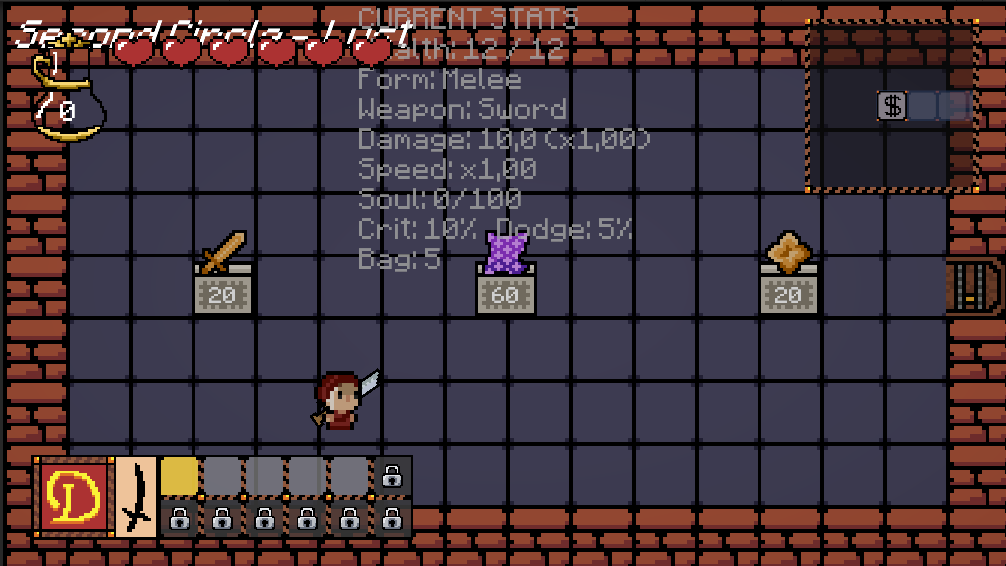
\includegraphics[width=.9\textwidth]{figures/resultados/iteracion7/19_sala_tienda.png}
\caption{Resultado de la feature Sala Tienda en la iteración 7}
\label{fig:iteracion7-feature-tienda}
\end{center}
\end{figure}

\begin{figure}[htbp]
\begin{center}
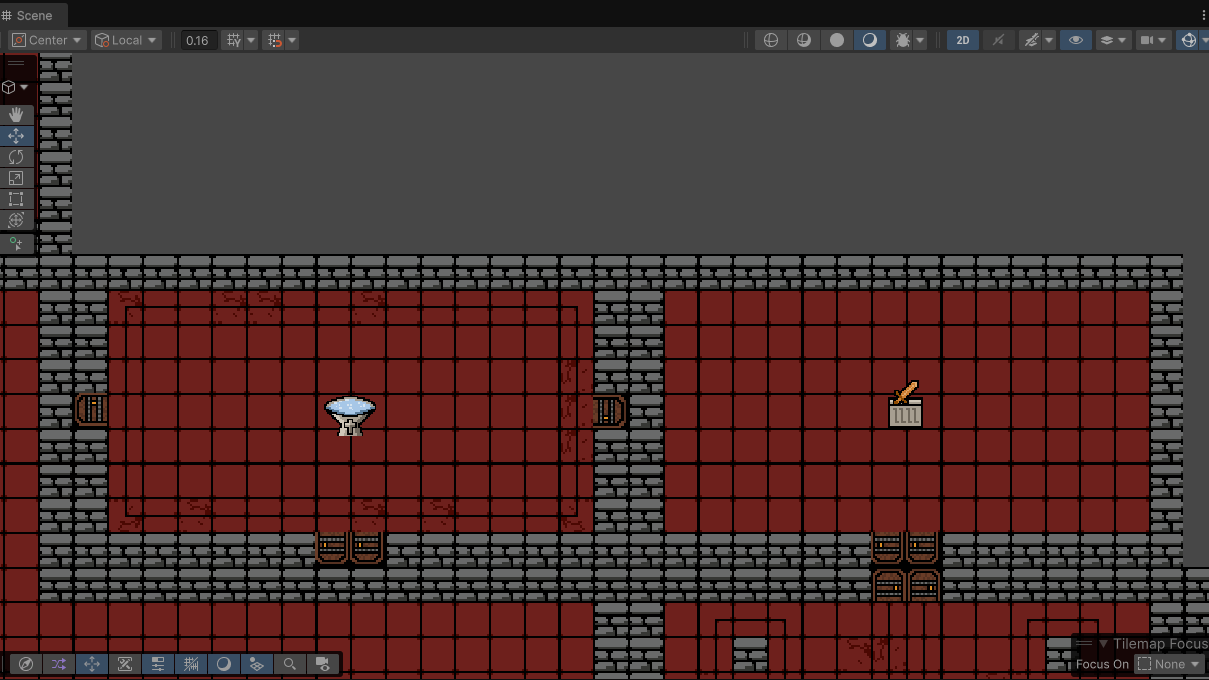
\includegraphics[width=.9\textwidth]{figures/resultados/iteracion7/20_sala_secreta_y_tesoro.png}
\caption{Resultado de la feature Sala Secreta y Tesoro en la iteración 7}
\label{fig:iteracion7-feature-salas-especiales}
\end{center}
\end{figure}

\begin{figure}[htbp]
\begin{center}
\includegraphics[width=.9\textwidth]{figures/resultados/iteracion7/21_sistema_combate_ii.png}
\caption{Resultado de la feature Sistema de Combate II en la iteración 7}
\label{fig:iteracion7-feature-combate}
\end{center}
\end{figure}

\begin{figure}[htbp]
\begin{center}
\includegraphics[width=.9\textwidth]{figures/resultados/iteracion7/22_sistema_enemigos_ii.png}
\caption{Resultado de la feature Sistema de Enemigos II en la iteración 7}
\label{fig:iteracion7-feature-enemigos}
\end{center}
\end{figure}

La Figura~\ref{fig:uml-resultado-iteracion7} recoge el diagrama UML de resultado de la iteración 7.

\begin{figure}[htbp]
\begin{center}
% \missingfigure{Sustituir por el diagrama UML de resultado de la iteración 7}
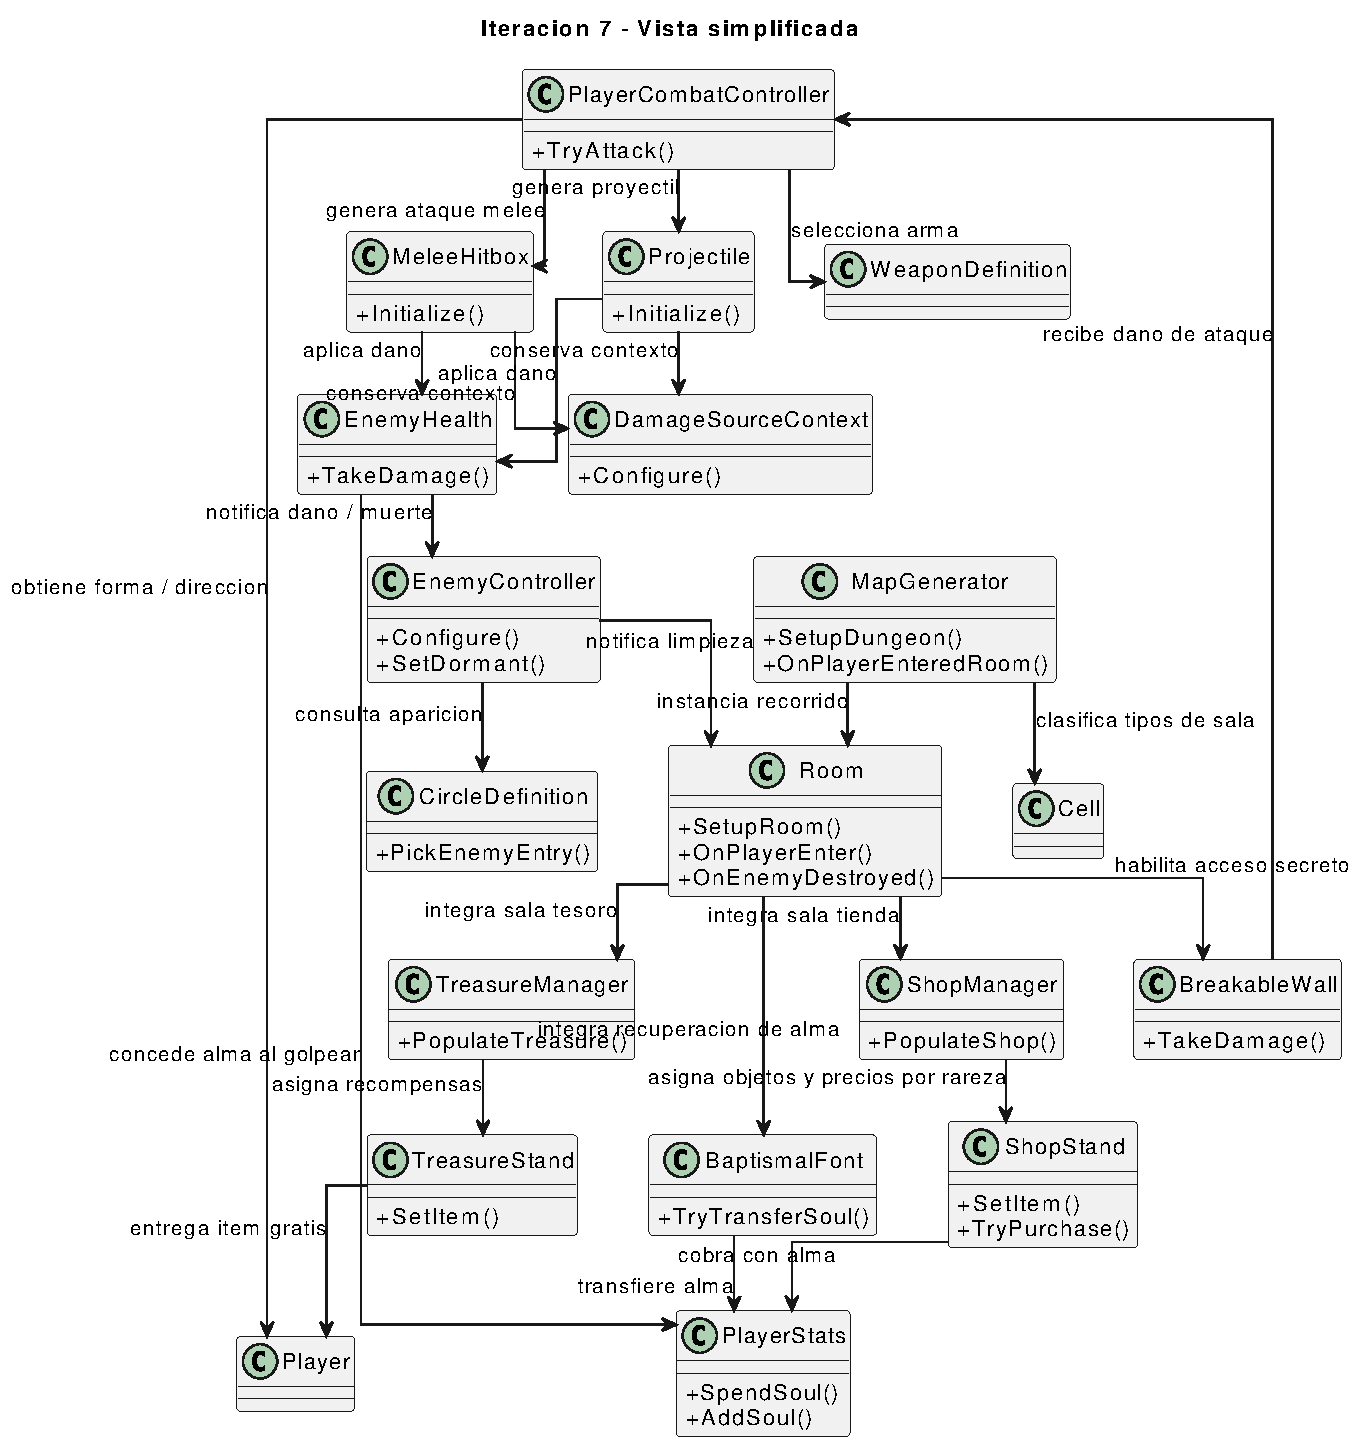
\includegraphics[width=\textwidth]{figures/iteracion7_resultado_uml.pdf}
\caption{Diagrama UML de resultado de la iteración 7}
\label{fig:uml-resultado-iteracion7}
\end{center}
\end{figure}
